\documentclass[]{article}
\usepackage{lmodern}
\usepackage{amssymb,amsmath}
\usepackage{ifxetex,ifluatex}
\usepackage{fixltx2e} % provides \textsubscript
\ifnum 0\ifxetex 1\fi\ifluatex 1\fi=0 % if pdftex
  \usepackage[T1]{fontenc}
  \usepackage[utf8]{inputenc}
\else % if luatex or xelatex
  \ifxetex
    \usepackage{mathspec}
  \else
    \usepackage{fontspec}
  \fi
  \defaultfontfeatures{Ligatures=TeX,Scale=MatchLowercase}
\fi
% use upquote if available, for straight quotes in verbatim environments
\IfFileExists{upquote.sty}{\usepackage{upquote}}{}
% use microtype if available
\IfFileExists{microtype.sty}{%
\usepackage[]{microtype}
\UseMicrotypeSet[protrusion]{basicmath} % disable protrusion for tt fonts
}{}
\PassOptionsToPackage{hyphens}{url} % url is loaded by hyperref
\usepackage[unicode=true]{hyperref}
\hypersetup{
            pdftitle={Radiomics},
            pdfborder={0 0 0},
            breaklinks=true}
\urlstyle{same}  % don't use monospace font for urls
\usepackage[margin=1in]{geometry}
\usepackage{color}
\usepackage{fancyvrb}
\newcommand{\VerbBar}{|}
\newcommand{\VERB}{\Verb[commandchars=\\\{\}]}
\DefineVerbatimEnvironment{Highlighting}{Verbatim}{commandchars=\\\{\}}
% Add ',fontsize=\small' for more characters per line
\usepackage{framed}
\definecolor{shadecolor}{RGB}{248,248,248}
\newenvironment{Shaded}{\begin{snugshade}}{\end{snugshade}}
\newcommand{\KeywordTok}[1]{\textcolor[rgb]{0.13,0.29,0.53}{\textbf{#1}}}
\newcommand{\DataTypeTok}[1]{\textcolor[rgb]{0.13,0.29,0.53}{#1}}
\newcommand{\DecValTok}[1]{\textcolor[rgb]{0.00,0.00,0.81}{#1}}
\newcommand{\BaseNTok}[1]{\textcolor[rgb]{0.00,0.00,0.81}{#1}}
\newcommand{\FloatTok}[1]{\textcolor[rgb]{0.00,0.00,0.81}{#1}}
\newcommand{\ConstantTok}[1]{\textcolor[rgb]{0.00,0.00,0.00}{#1}}
\newcommand{\CharTok}[1]{\textcolor[rgb]{0.31,0.60,0.02}{#1}}
\newcommand{\SpecialCharTok}[1]{\textcolor[rgb]{0.00,0.00,0.00}{#1}}
\newcommand{\StringTok}[1]{\textcolor[rgb]{0.31,0.60,0.02}{#1}}
\newcommand{\VerbatimStringTok}[1]{\textcolor[rgb]{0.31,0.60,0.02}{#1}}
\newcommand{\SpecialStringTok}[1]{\textcolor[rgb]{0.31,0.60,0.02}{#1}}
\newcommand{\ImportTok}[1]{#1}
\newcommand{\CommentTok}[1]{\textcolor[rgb]{0.56,0.35,0.01}{\textit{#1}}}
\newcommand{\DocumentationTok}[1]{\textcolor[rgb]{0.56,0.35,0.01}{\textbf{\textit{#1}}}}
\newcommand{\AnnotationTok}[1]{\textcolor[rgb]{0.56,0.35,0.01}{\textbf{\textit{#1}}}}
\newcommand{\CommentVarTok}[1]{\textcolor[rgb]{0.56,0.35,0.01}{\textbf{\textit{#1}}}}
\newcommand{\OtherTok}[1]{\textcolor[rgb]{0.56,0.35,0.01}{#1}}
\newcommand{\FunctionTok}[1]{\textcolor[rgb]{0.00,0.00,0.00}{#1}}
\newcommand{\VariableTok}[1]{\textcolor[rgb]{0.00,0.00,0.00}{#1}}
\newcommand{\ControlFlowTok}[1]{\textcolor[rgb]{0.13,0.29,0.53}{\textbf{#1}}}
\newcommand{\OperatorTok}[1]{\textcolor[rgb]{0.81,0.36,0.00}{\textbf{#1}}}
\newcommand{\BuiltInTok}[1]{#1}
\newcommand{\ExtensionTok}[1]{#1}
\newcommand{\PreprocessorTok}[1]{\textcolor[rgb]{0.56,0.35,0.01}{\textit{#1}}}
\newcommand{\AttributeTok}[1]{\textcolor[rgb]{0.77,0.63,0.00}{#1}}
\newcommand{\RegionMarkerTok}[1]{#1}
\newcommand{\InformationTok}[1]{\textcolor[rgb]{0.56,0.35,0.01}{\textbf{\textit{#1}}}}
\newcommand{\WarningTok}[1]{\textcolor[rgb]{0.56,0.35,0.01}{\textbf{\textit{#1}}}}
\newcommand{\AlertTok}[1]{\textcolor[rgb]{0.94,0.16,0.16}{#1}}
\newcommand{\ErrorTok}[1]{\textcolor[rgb]{0.64,0.00,0.00}{\textbf{#1}}}
\newcommand{\NormalTok}[1]{#1}
\usepackage{graphicx,grffile}
\makeatletter
\def\maxwidth{\ifdim\Gin@nat@width>\linewidth\linewidth\else\Gin@nat@width\fi}
\def\maxheight{\ifdim\Gin@nat@height>\textheight\textheight\else\Gin@nat@height\fi}
\makeatother
% Scale images if necessary, so that they will not overflow the page
% margins by default, and it is still possible to overwrite the defaults
% using explicit options in \includegraphics[width, height, ...]{}
\setkeys{Gin}{width=\maxwidth,height=\maxheight,keepaspectratio}
\IfFileExists{parskip.sty}{%
\usepackage{parskip}
}{% else
\setlength{\parindent}{0pt}
\setlength{\parskip}{6pt plus 2pt minus 1pt}
}
\setlength{\emergencystretch}{3em}  % prevent overfull lines
\providecommand{\tightlist}{%
  \setlength{\itemsep}{0pt}\setlength{\parskip}{0pt}}
\setcounter{secnumdepth}{0}
% Redefines (sub)paragraphs to behave more like sections
\ifx\paragraph\undefined\else
\let\oldparagraph\paragraph
\renewcommand{\paragraph}[1]{\oldparagraph{#1}\mbox{}}
\fi
\ifx\subparagraph\undefined\else
\let\oldsubparagraph\subparagraph
\renewcommand{\subparagraph}[1]{\oldsubparagraph{#1}\mbox{}}
\fi

% set default figure placement to htbp
\makeatletter
\def\fps@figure{htbp}
\makeatother


\title{Radiomics}
\author{}
\date{\vspace{-2.5em}}

\begin{document}
\maketitle

\section{Loading Everything}\label{loading-everything}

\section{Project Plan}\label{project-plan}

\begin{figure}
\centering
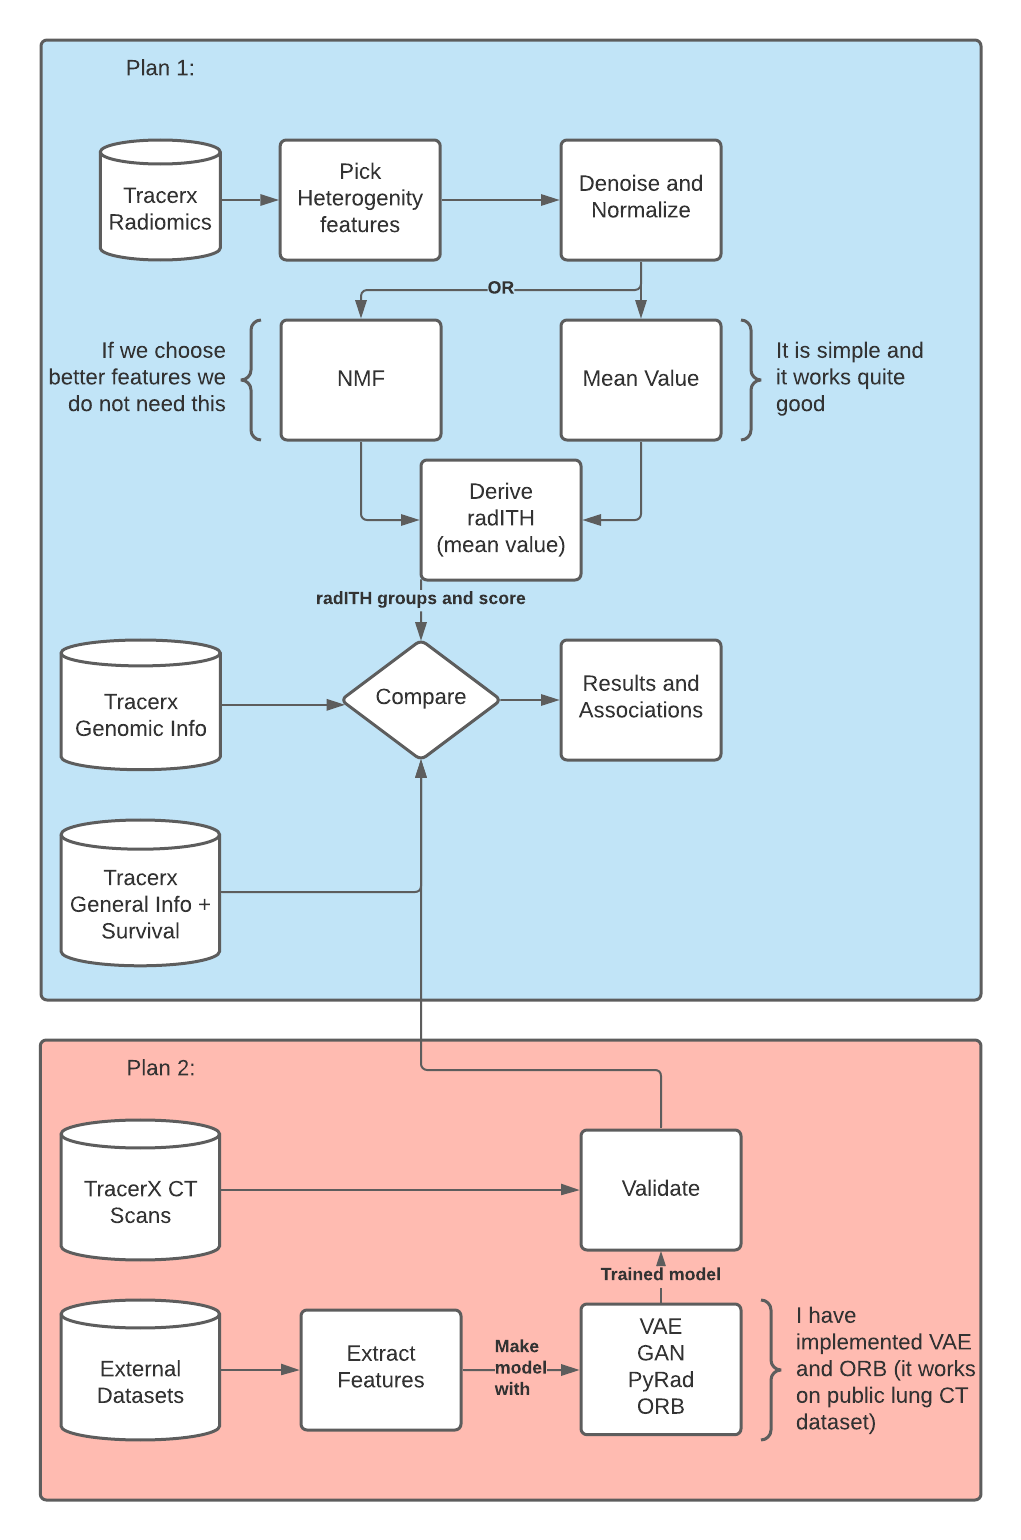
\includegraphics{~/GenomeDK_local/CancerEvolution/phd/Analysis/radiomics/NMF_Radiomics/Radiomics.png}
\caption{Project Plan}
\end{figure}

\section{What features to take?}\label{what-features-to-take}

-Not sure to take Zone Entropy or not\\
-Run Entropy and Zone Entropy do not follow the same patter on biplot\\
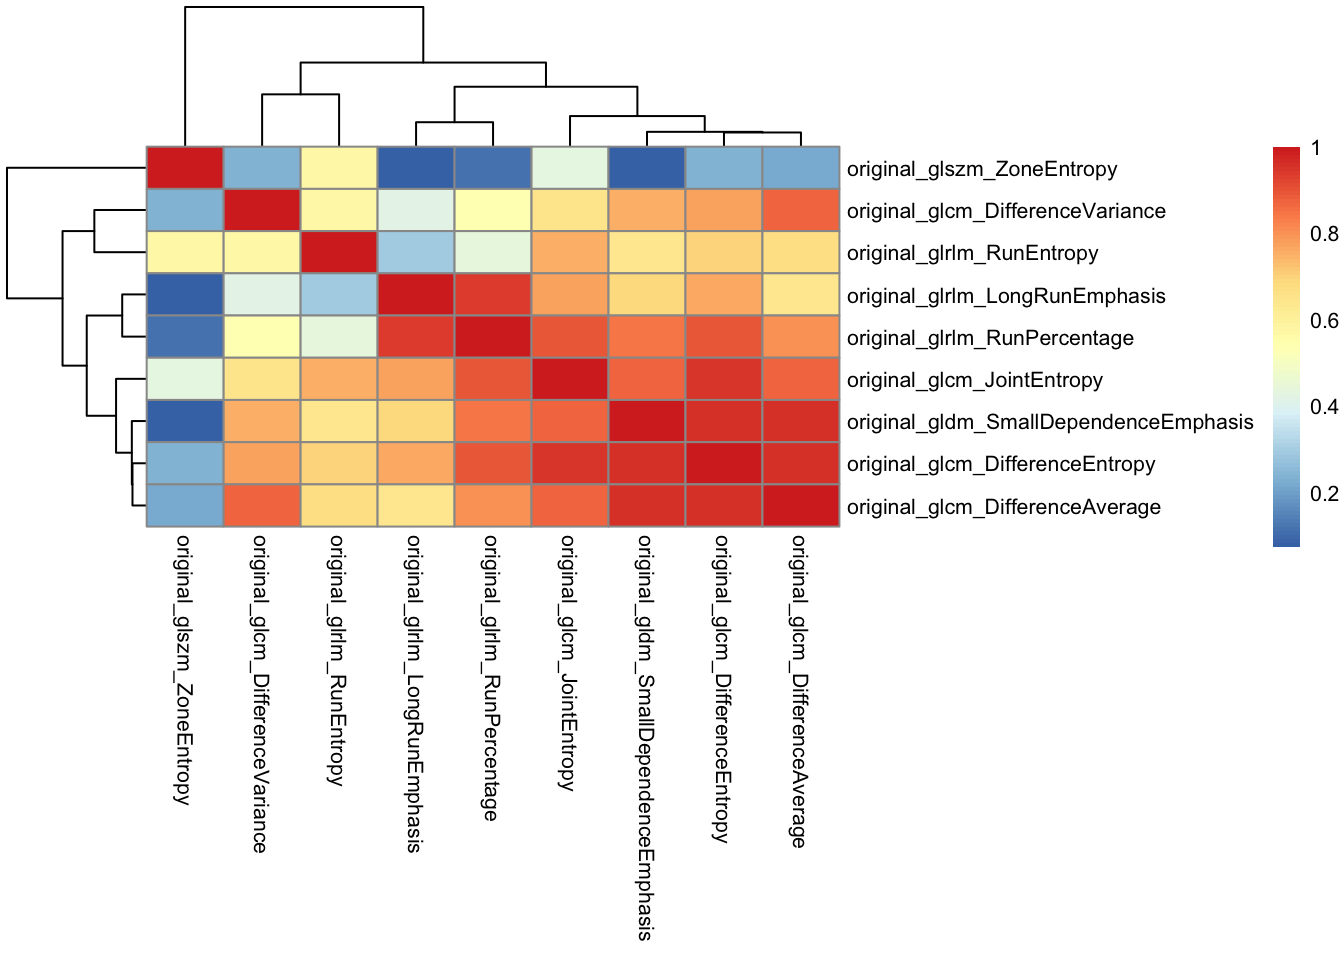
\includegraphics{radiomics_USA_January_2022_files/figure-latex/unnamed-chunk-2-1.pdf}
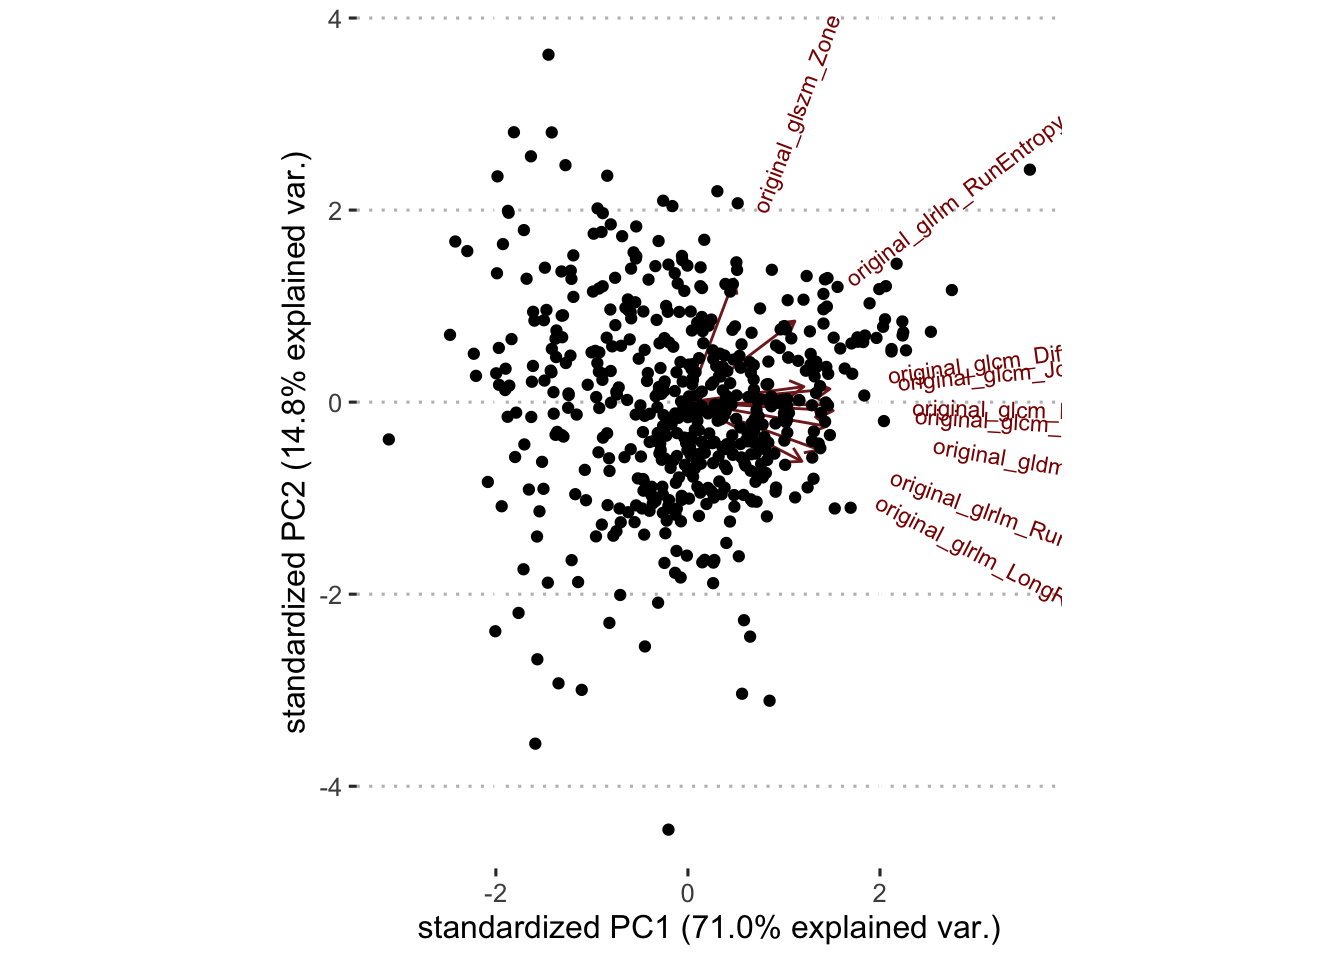
\includegraphics{radiomics_USA_January_2022_files/figure-latex/unnamed-chunk-2-2.pdf}

\section{Important measures to check}\label{important-measures-to-check}

-We will compare diameter to volume to ITH\\

\begin{Shaded}
\begin{Highlighting}[]
\NormalTok{pyrad}\OperatorTok{$}\NormalTok{volume =}\StringTok{ }\KeywordTok{as.numeric}\NormalTok{(pyrad}\OperatorTok{$}\NormalTok{lesion1sizepath)}
\NormalTok{pyrad}\OperatorTok{$}\NormalTok{volume_from_pyrad =}\StringTok{ }\KeywordTok{as.numeric}\NormalTok{(pyrad}\OperatorTok{$}\NormalTok{original_shape_MeshVolume)}
\NormalTok{pyrad}\OperatorTok{$}\NormalTok{diameter =}\StringTok{ }\KeywordTok{as.numeric}\NormalTok{(pyrad}\OperatorTok{$}\NormalTok{original_shape_Maximum2DDiameterSlice)}
\end{Highlighting}
\end{Shaded}

\section{how to define radITH}\label{how-to-define-radith}

-Do we need to normalize something by volume?\\
-Numbers were a bit wierd when divided by volume therefore I did not
divide anything with volume

\begin{Shaded}
\begin{Highlighting}[]
\NormalTok{pyrad}\OperatorTok{$}\NormalTok{radITH =}\StringTok{ }\KeywordTok{rowMeans}\NormalTok{(pyrad[,features_of_interest], }\DataTypeTok{na.rm =}\NormalTok{ T)}
\NormalTok{Q =}\StringTok{ }\DecValTok{3}


\NormalTok{pyrad}\OperatorTok{$}\NormalTok{volume_group =}\StringTok{ }\NormalTok{gtools}\OperatorTok{::}\KeywordTok{quantcut}\NormalTok{(pyrad}\OperatorTok{$}\NormalTok{volume, }\DataTypeTok{q=}\NormalTok{Q, }\DataTypeTok{na.rm=}\OtherTok{TRUE}\NormalTok{)}
\NormalTok{pyrad}\OperatorTok{$}\NormalTok{diameter_group =}\StringTok{ }\NormalTok{gtools}\OperatorTok{::}\KeywordTok{quantcut}\NormalTok{(pyrad}\OperatorTok{$}\NormalTok{diameter, }\DataTypeTok{q=}\NormalTok{Q, }\DataTypeTok{na.rm=}\OtherTok{TRUE}\NormalTok{)}
\NormalTok{pyrad}\OperatorTok{$}\NormalTok{radITH_group =}\StringTok{ }\NormalTok{gtools}\OperatorTok{::}\KeywordTok{quantcut}\NormalTok{(pyrad}\OperatorTok{$}\NormalTok{radITH, }\DataTypeTok{q=}\NormalTok{Q, }\DataTypeTok{na.rm=}\OtherTok{TRUE}\NormalTok{)}
\end{Highlighting}
\end{Shaded}

\section{Expected correlations}\label{expected-correlations}

-Negative cor radITH to volume\\
-Positive cor to ORACLE(not true)\\
-Volume and diameter are correlated to volume therefore we are probably
not confunded by volume\\
-We would expect poz. cor. to Heterogenious but not mandatory since we
do not know if radITH is the same as bioITH\\
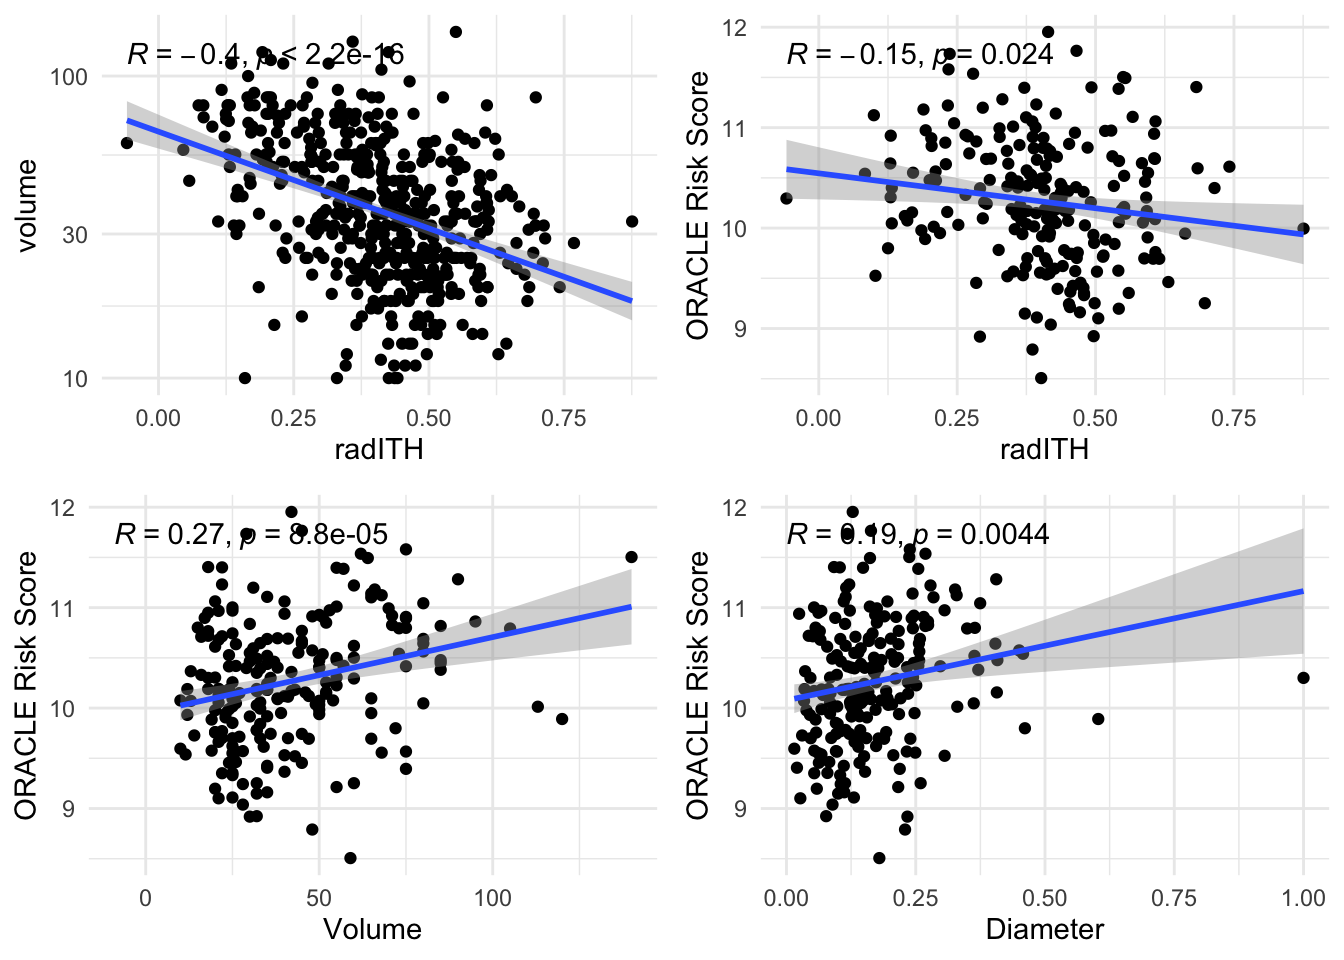
\includegraphics{radiomics_USA_January_2022_files/figure-latex/unnamed-chunk-5-1.pdf}
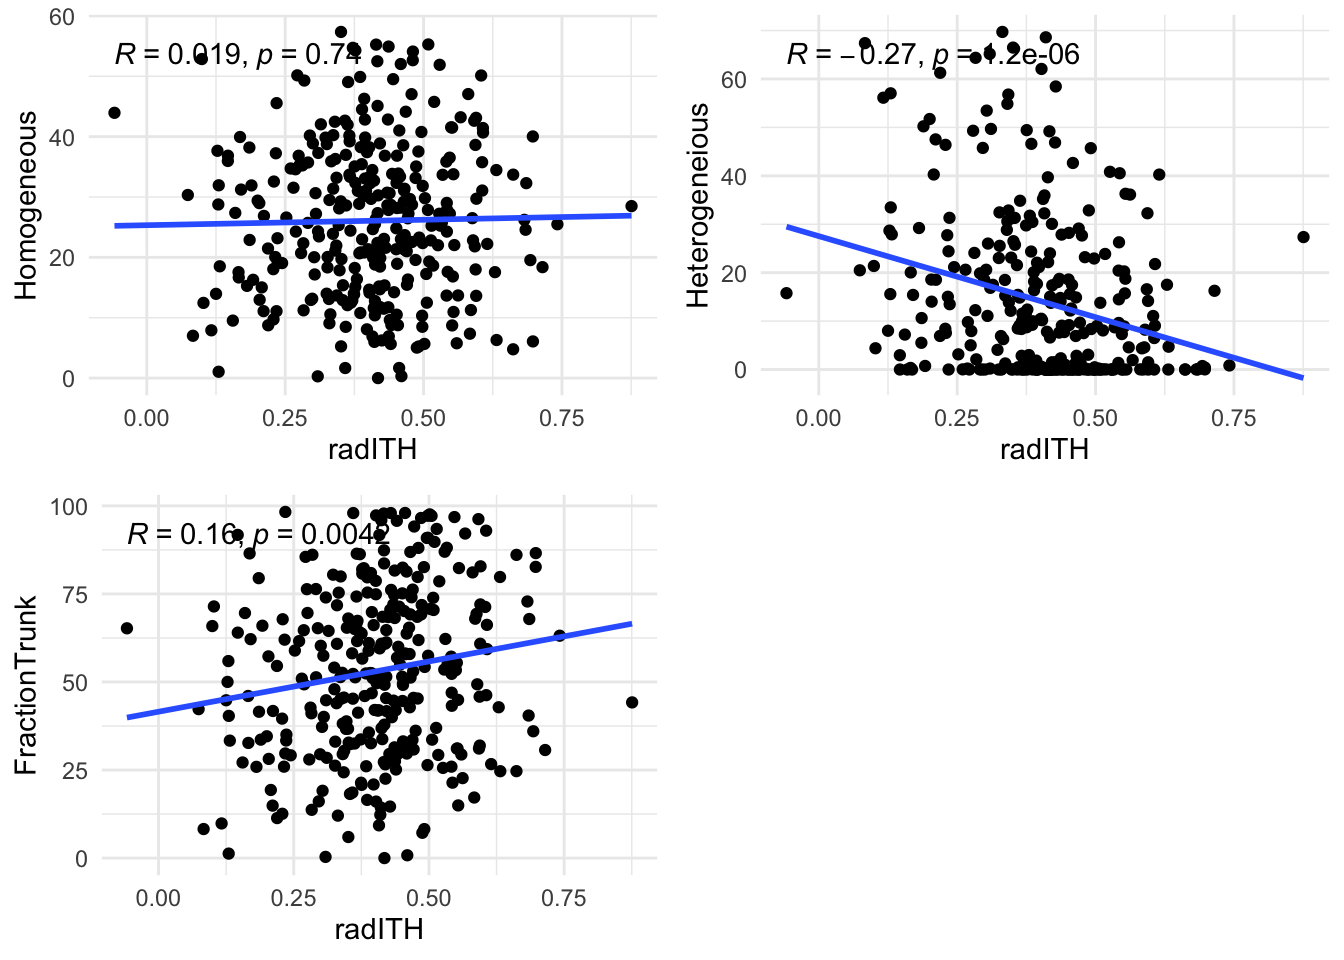
\includegraphics{radiomics_USA_January_2022_files/figure-latex/unnamed-chunk-5-2.pdf}

\section{Mutations}\label{mutations}

Let's group DRIVER mutations by Sanchez Vega def\\
\ldots{}

\section{Let's test Sanchez Vega Muts vs radITH groups (q
=3)}\label{lets-test-sanchez-vega-muts-vs-radith-groups-q-3}

-It seems Adeno is associated with wtn, cell\_cycle,pi3k\\
-It seems Squamous is associated with pi3k and RTK/KRAS\\

\begin{verbatim}
## [1] "Adeno fisher test results"
\end{verbatim}

\begin{verbatim}
## [1] "nrf2"
## 
##  Fisher's Exact Test for Count Data
## 
## data:  table(tmp$radITH_group, tmp[, col])
## p-value = 0.02679
## alternative hypothesis: two.sided
## 
## [1] "pi3k"
## 
##  Fisher's Exact Test for Count Data
## 
## data:  table(tmp$radITH_group, tmp[, col])
## p-value = 0.003382
## alternative hypothesis: two.sided
## 
## [1] "cell_cycle"
## 
##  Fisher's Exact Test for Count Data
## 
## data:  table(tmp$radITH_group, tmp[, col])
## p-value = 0.0003902
## alternative hypothesis: two.sided
## 
## [1] "wnt"
## 
##  Fisher's Exact Test for Count Data
## 
## data:  table(tmp$radITH_group, tmp[, col])
## p-value = 0.04017
## alternative hypothesis: two.sided
\end{verbatim}

\begin{verbatim}
## [1] "Squamous fisher test results"
\end{verbatim}

\begin{verbatim}
## [1] "rtk_kras"
## 
##  Fisher's Exact Test for Count Data
## 
## data:  table(tmp$radITH_group, tmp[, col])
## p-value = 0.01748
## alternative hypothesis: two.sided
## 
## [1] "pi3k"
## 
##  Fisher's Exact Test for Count Data
## 
## data:  table(tmp$radITH_group, tmp[, col])
## p-value = 0.007167
## alternative hypothesis: two.sided
\end{verbatim}

\section{Does Volume or diameter predict
biology?}\label{does-volume-or-diameter-predict-biology}

-Diameter is not associated at all\\
-Volume is associated with HIPPO\\

\begin{verbatim}
## [1] "Adeno fisher test results"
\end{verbatim}

\begin{verbatim}
## [1] "Squamous fisher test results"
\end{verbatim}

\begin{verbatim}
## [1] "hippo"
## 
##  Fisher's Exact Test for Count Data
## 
## data:  table(tmp$volume_group, tmp[, col])
## p-value = 0.01164
## alternative hypothesis: two.sided
\end{verbatim}

\section{How does radITH associate with
survival?}\label{how-does-radith-associate-with-survival}

-In Adeno Heterogenious tumors seem to perform better\\
-In Squamous no association\\
-In all samples, heterogenious samples seem to perform better\\
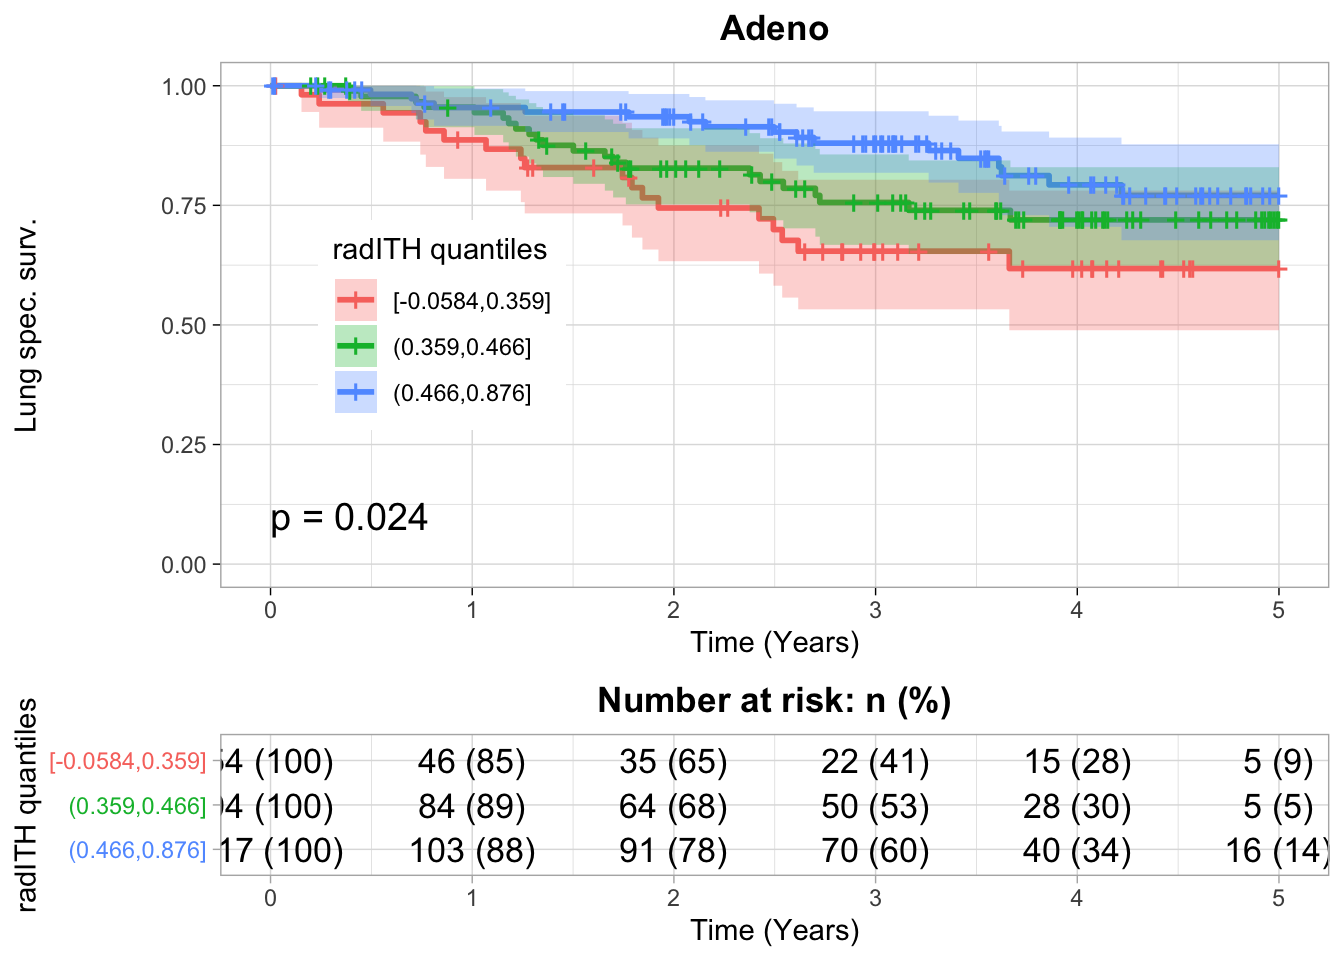
\includegraphics{radiomics_USA_January_2022_files/figure-latex/unnamed-chunk-9-1.pdf}
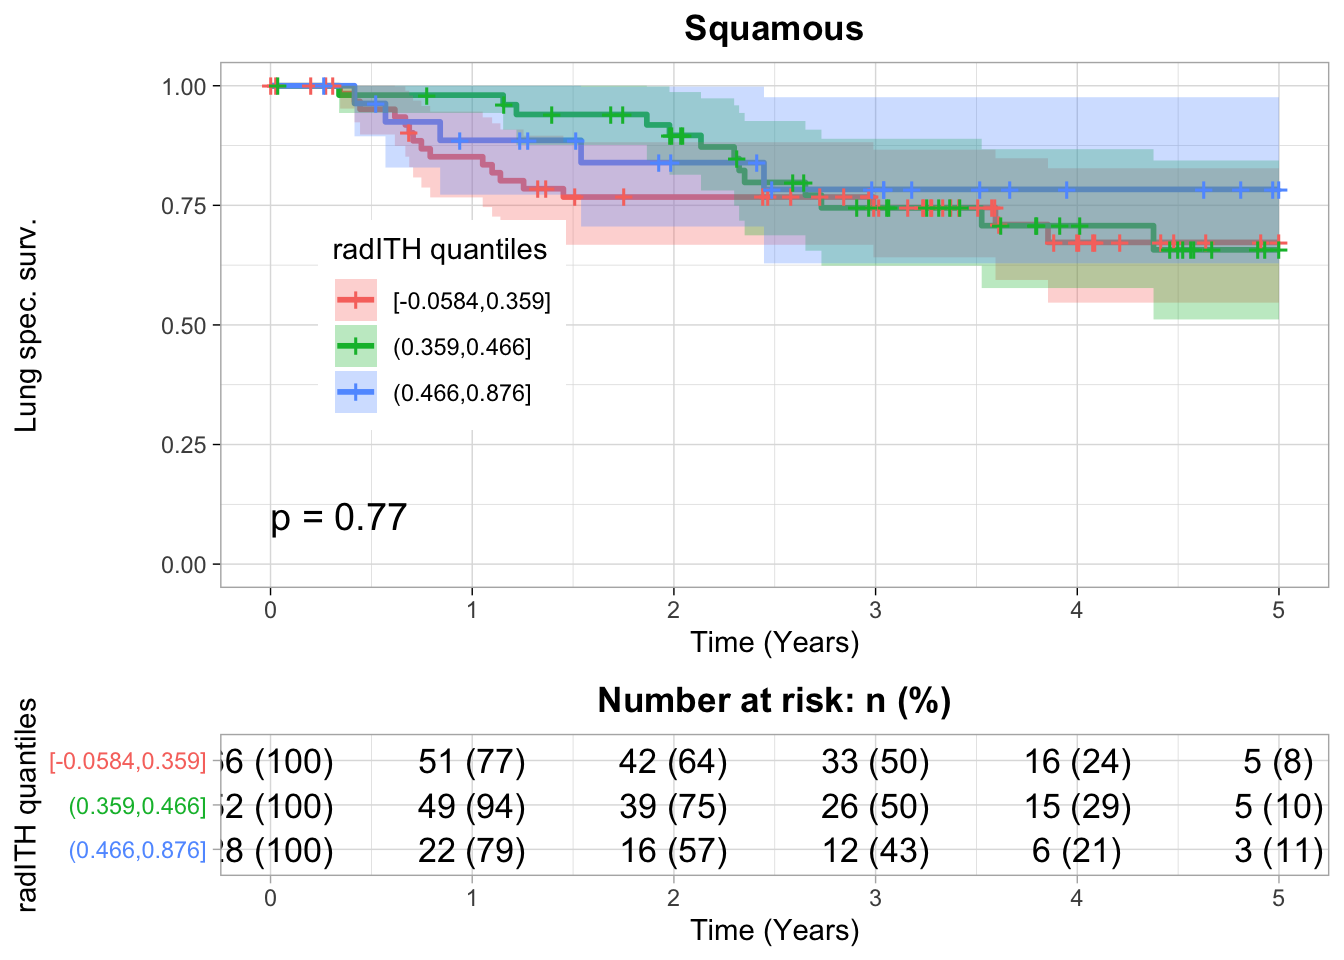
\includegraphics{radiomics_USA_January_2022_files/figure-latex/unnamed-chunk-9-2.pdf}
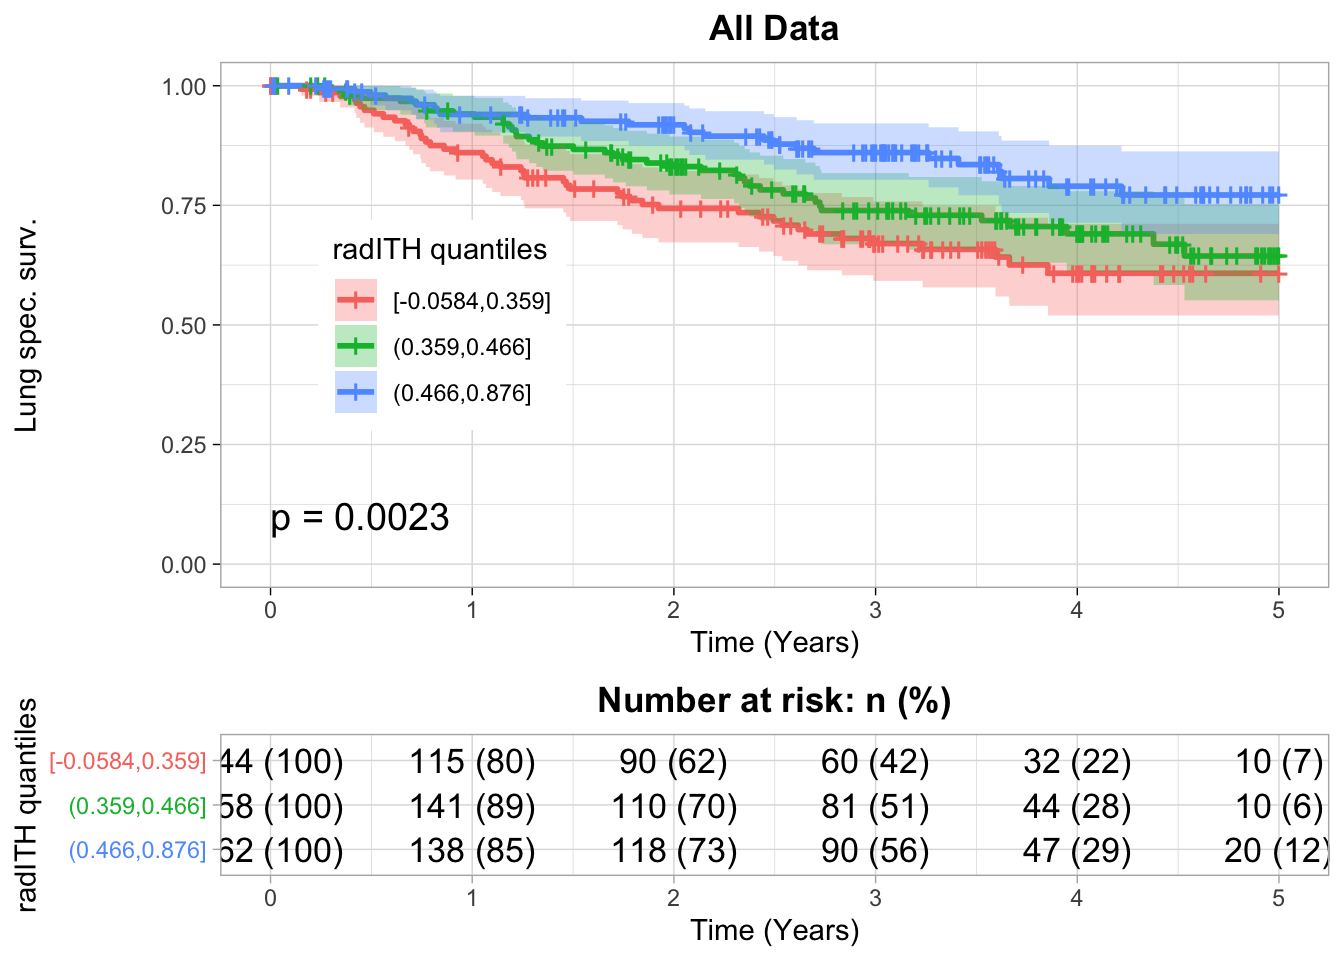
\includegraphics{radiomics_USA_January_2022_files/figure-latex/unnamed-chunk-9-3.pdf}

\section{How does volume (diameter) associate to
survival?}\label{how-does-volume-diameter-associate-to-survival}

-In Adeno large tumors seem to perform the worst(diamter is the same)\\
-In Squamous, volume has no clear association\\
-In Squamous, Diameter has borderline association\\
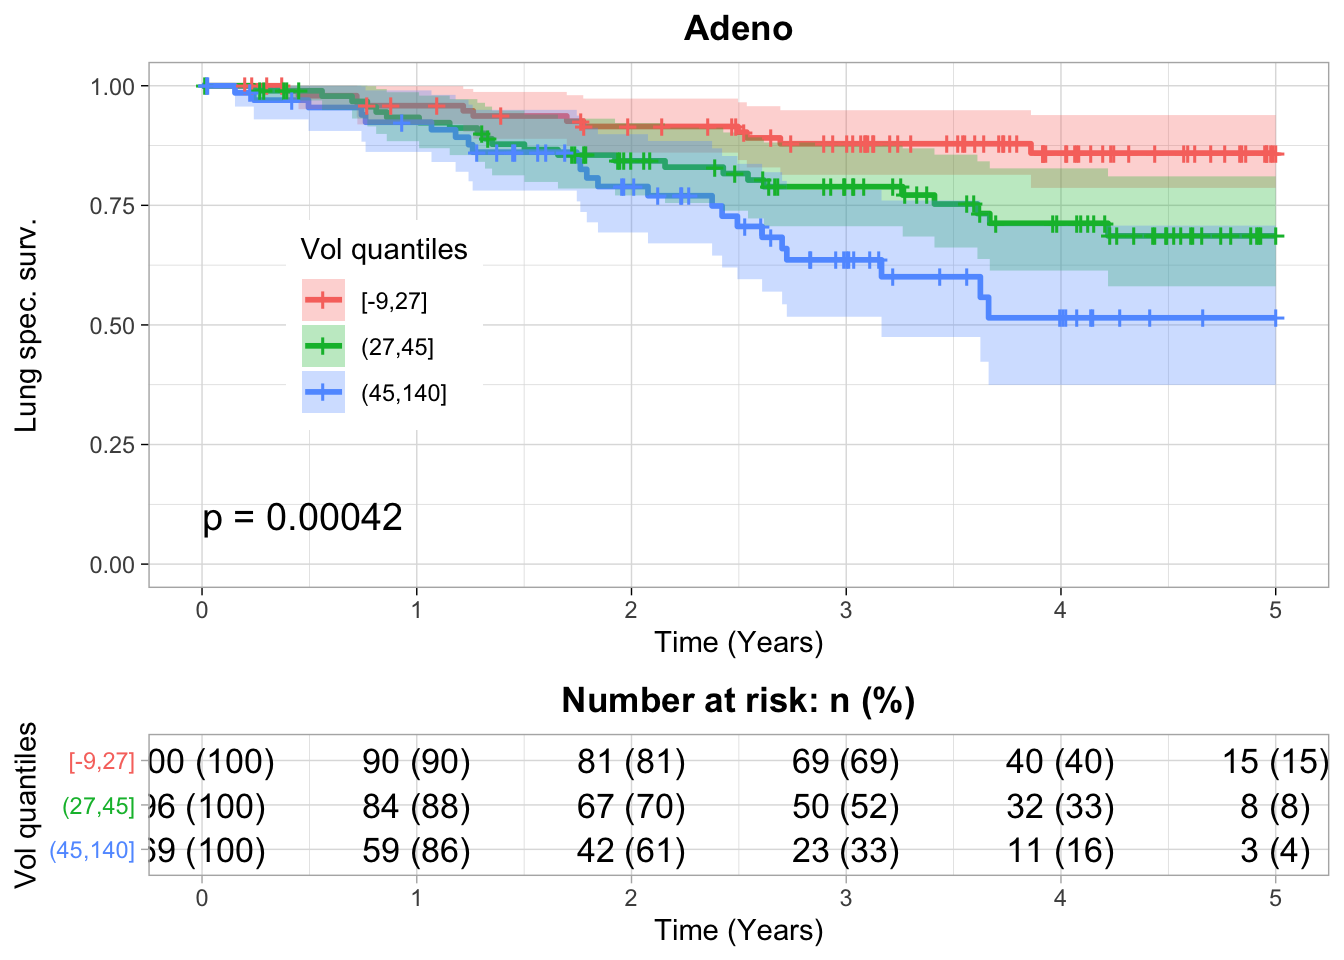
\includegraphics{radiomics_USA_January_2022_files/figure-latex/unnamed-chunk-10-1.pdf}
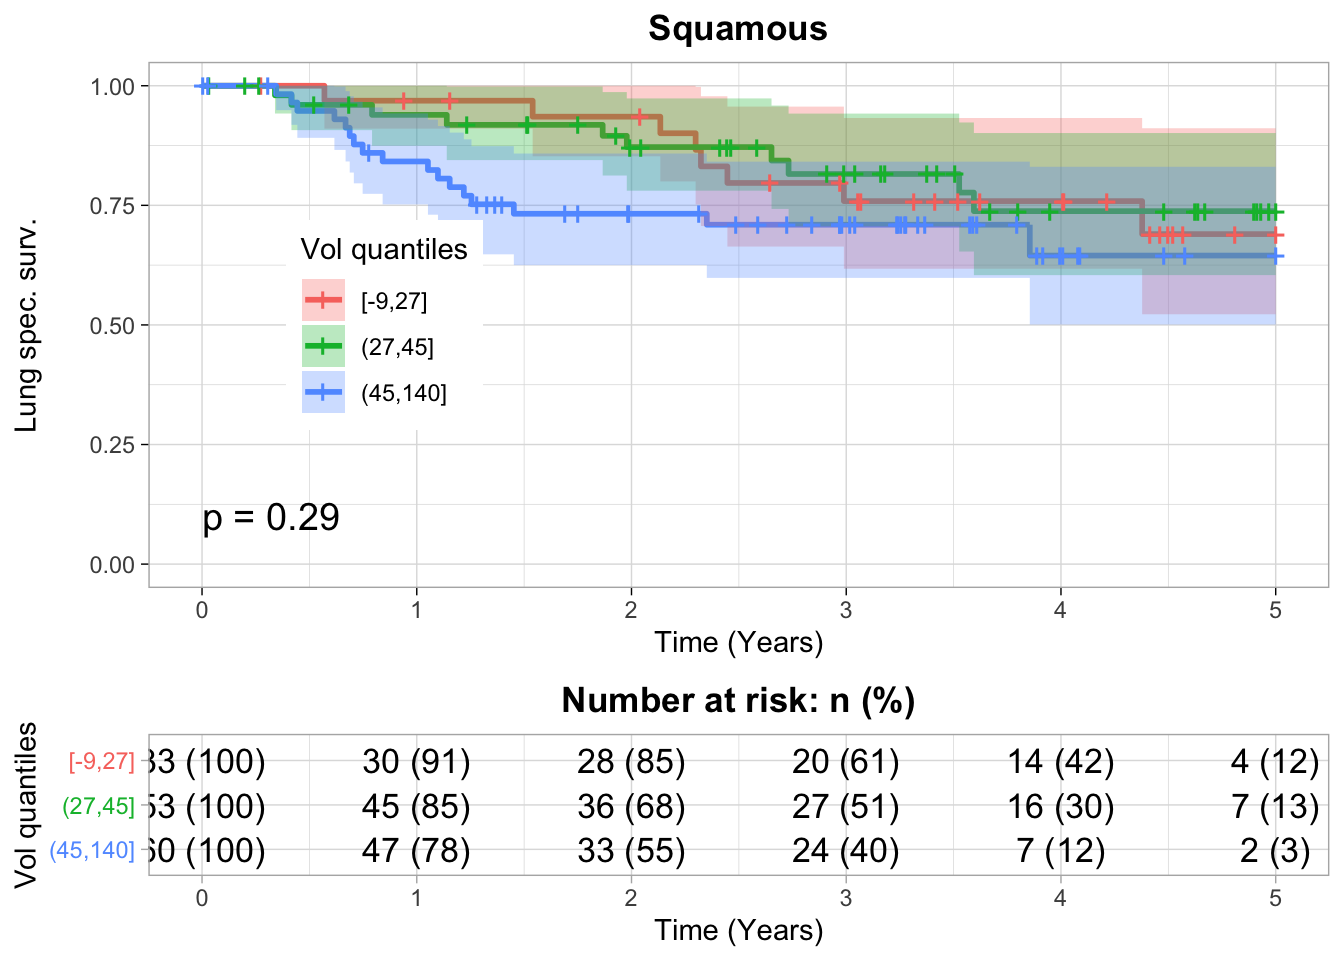
\includegraphics{radiomics_USA_January_2022_files/figure-latex/unnamed-chunk-10-2.pdf}
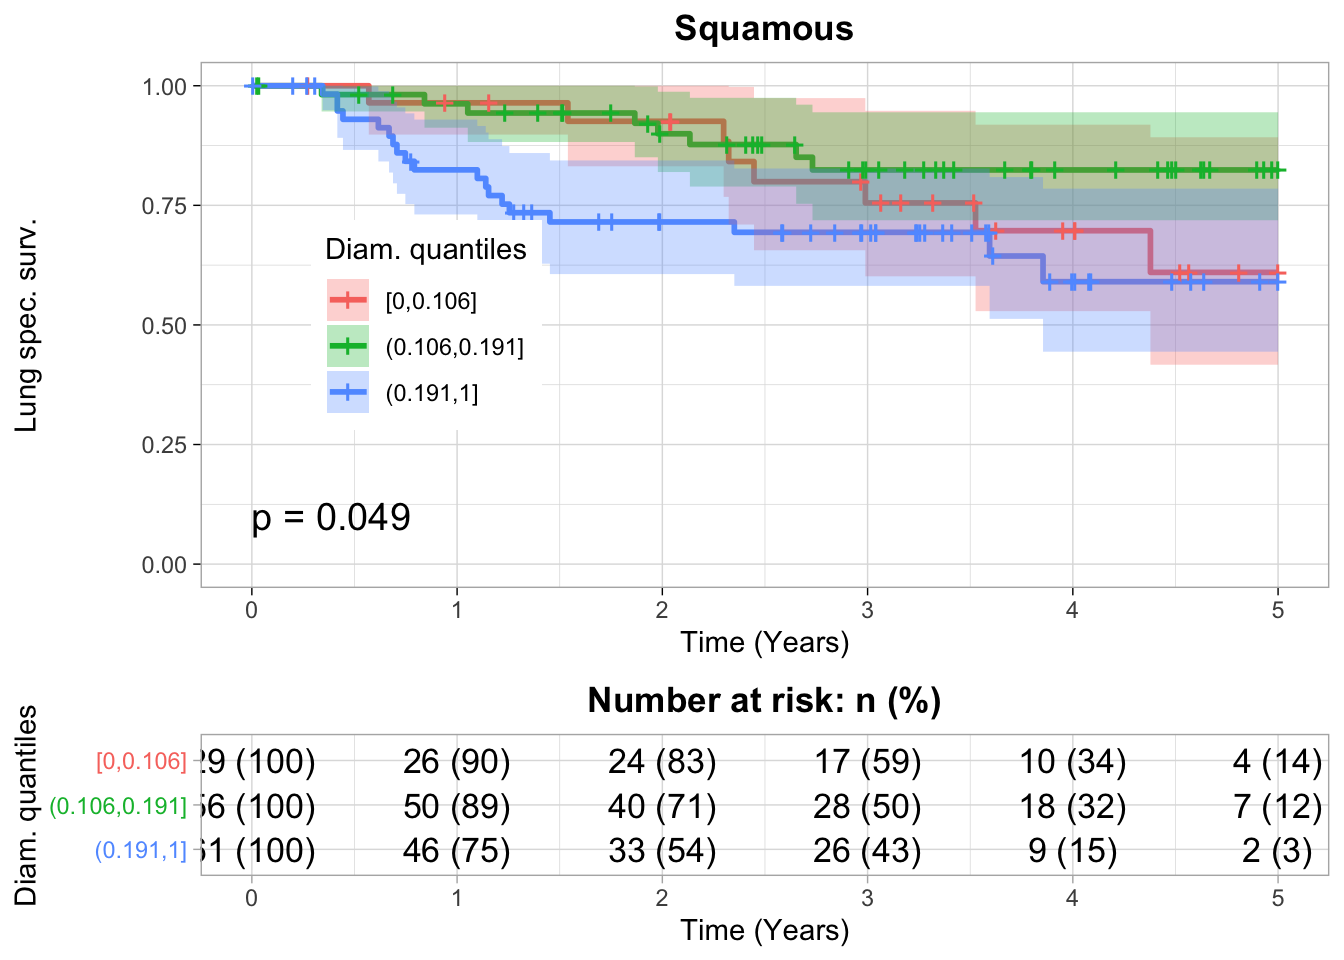
\includegraphics{radiomics_USA_January_2022_files/figure-latex/unnamed-chunk-10-3.pdf}

\section{Can we overlap radITH and Volume groups and check
survival?}\label{can-we-overlap-radith-and-volume-groups-and-check-survival}

\section{In order to increase group sizes, all measures will be split by
median
(Q=2)}\label{in-order-to-increase-group-sizes-all-measures-will-be-split-by-median-q2}

-Median was calculated based on entire cohort(not per cancer type)\\
-In Adeno, big tumors with low radITH seem to perform the worst where
small tumors with high radITH perform good(The same goes using
radITH-Diameter split)\\
-In Squmous we cannot see clear split(The same using radITH-diameter
split)\\
-In all data we see the similar pattern as in Adeno\\

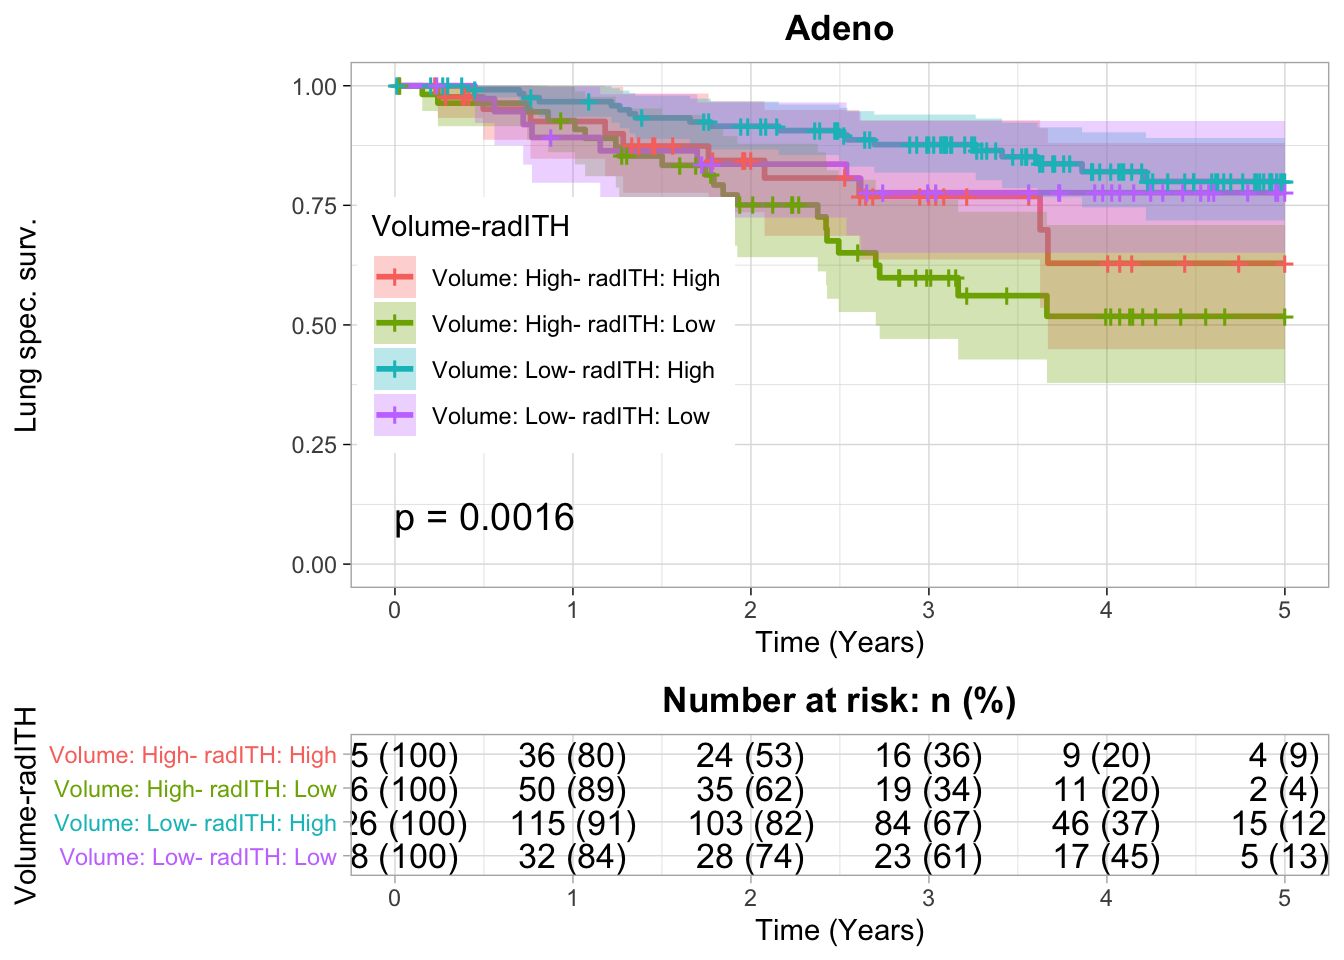
\includegraphics{radiomics_USA_January_2022_files/figure-latex/unnamed-chunk-11-1.pdf}
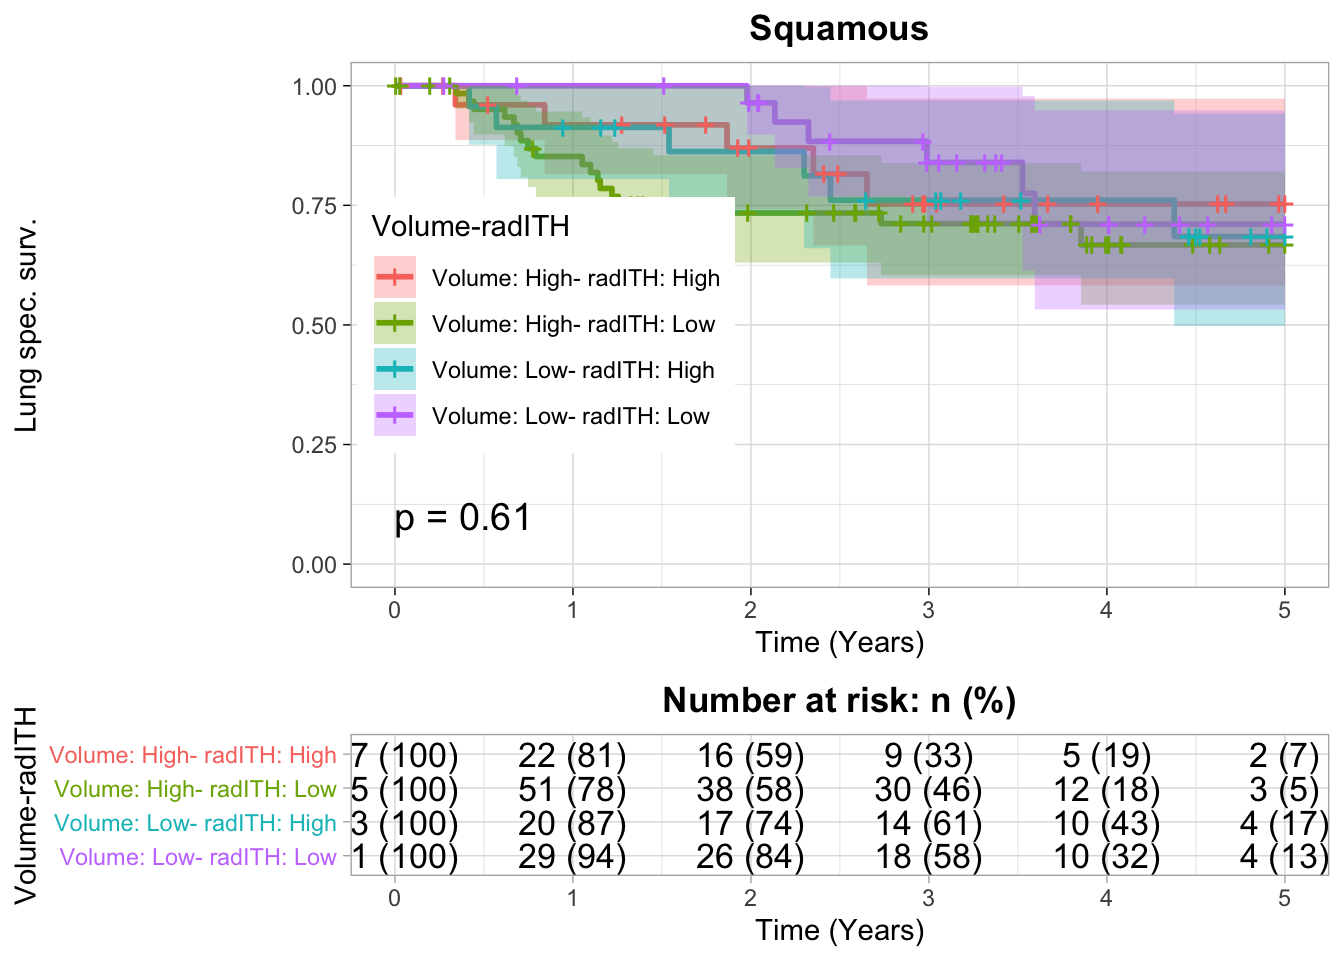
\includegraphics{radiomics_USA_January_2022_files/figure-latex/unnamed-chunk-11-2.pdf}
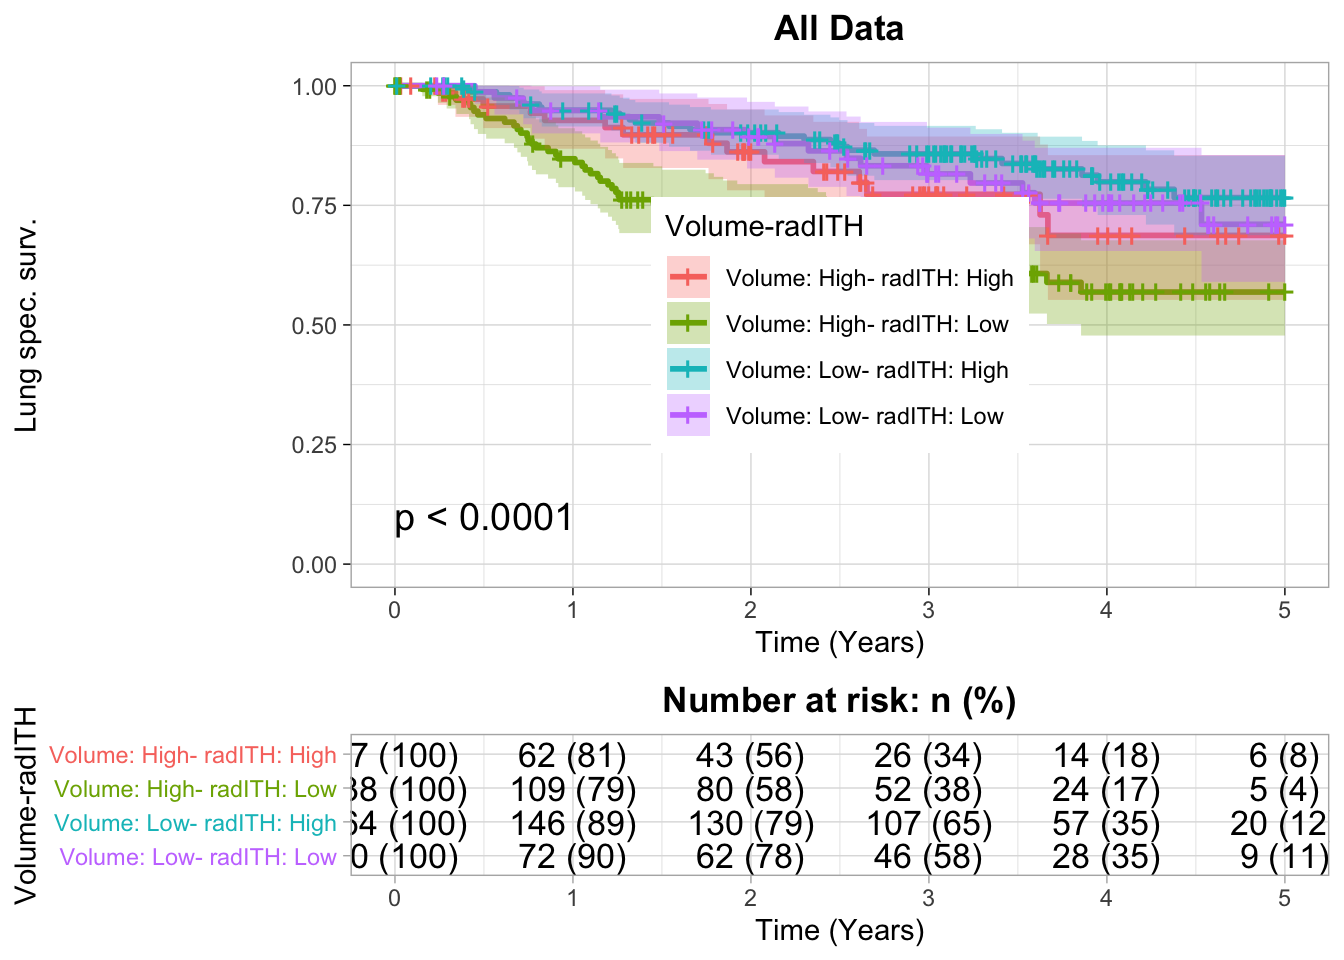
\includegraphics{radiomics_USA_January_2022_files/figure-latex/unnamed-chunk-11-3.pdf}

\section{Coxph Model}\label{coxph-model}

\begin{itemize}
\tightlist
\item
  radITH does not help improve cox ph model
  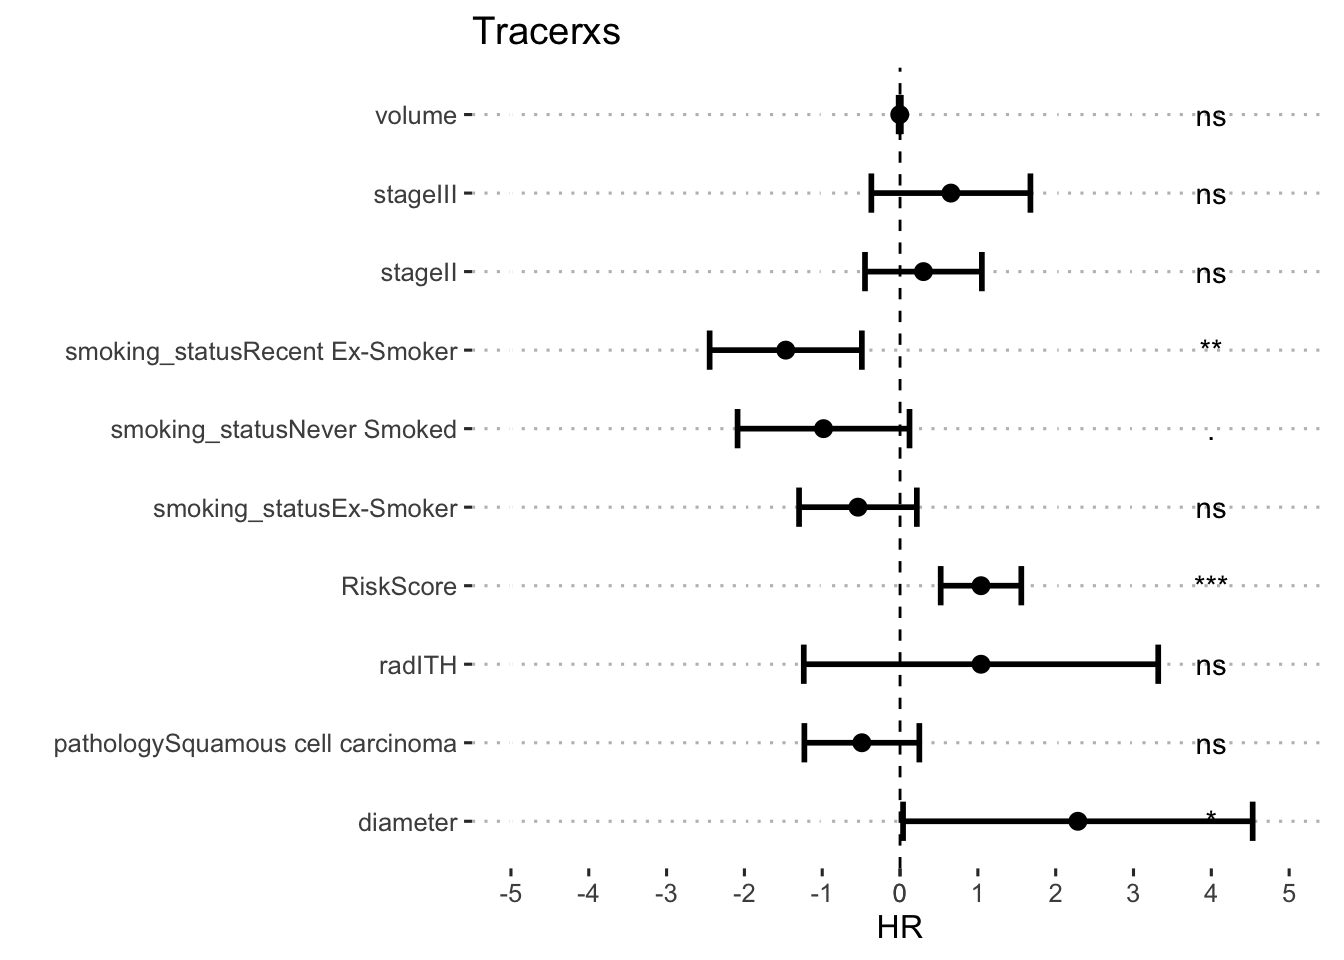
\includegraphics{radiomics_USA_January_2022_files/figure-latex/unnamed-chunk-12-1.pdf}
\end{itemize}

\section{Hallmarks all samples}\label{hallmarks-all-samples}

\begin{itemize}
\tightlist
\item
  Association of radITH with hallmarks\\
\item
  Hallmarks computed with SS-GSEA and GSVA
\item
  P values are adjusted using FDR\\
\end{itemize}

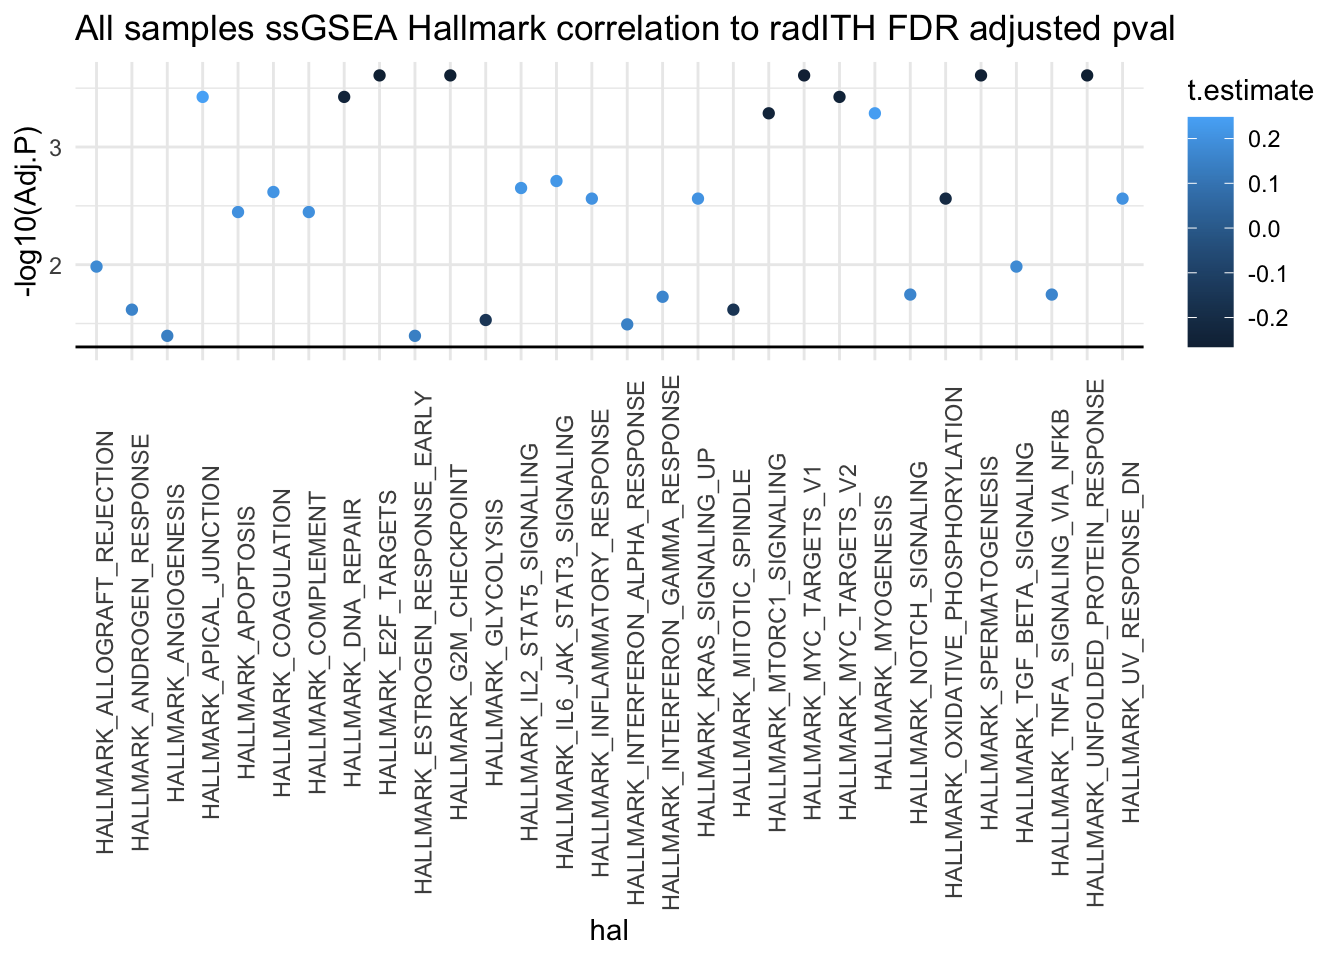
\includegraphics{radiomics_USA_January_2022_files/figure-latex/unnamed-chunk-13-1.pdf}
\# Hallmarks Adeno -No significant correlations\\
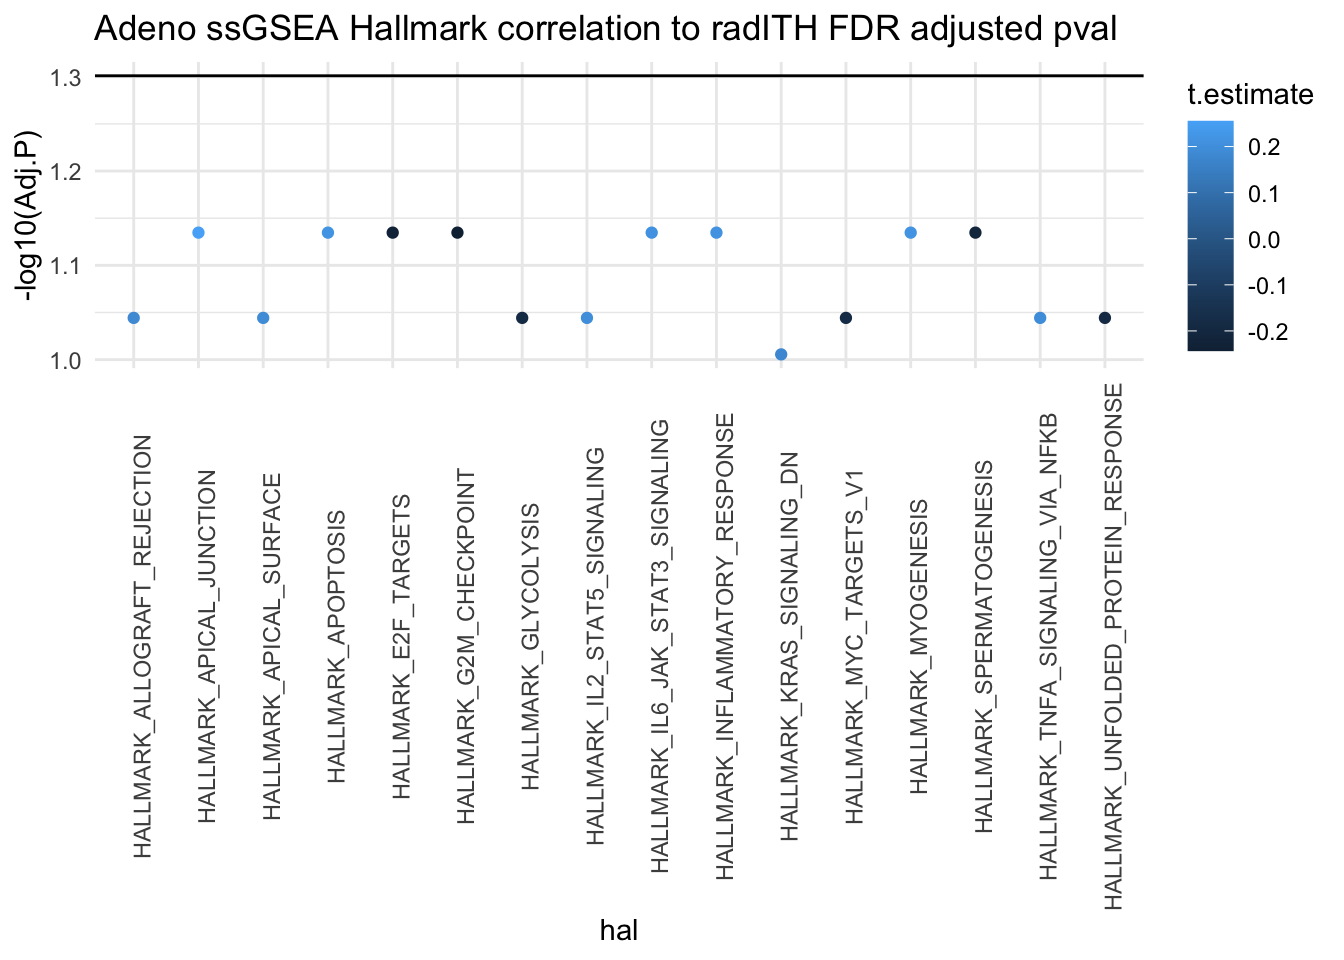
\includegraphics{radiomics_USA_January_2022_files/figure-latex/unnamed-chunk-14-1.pdf}

\section{Hallmarks Squamous}\label{hallmarks-squamous}

-No significant correlations
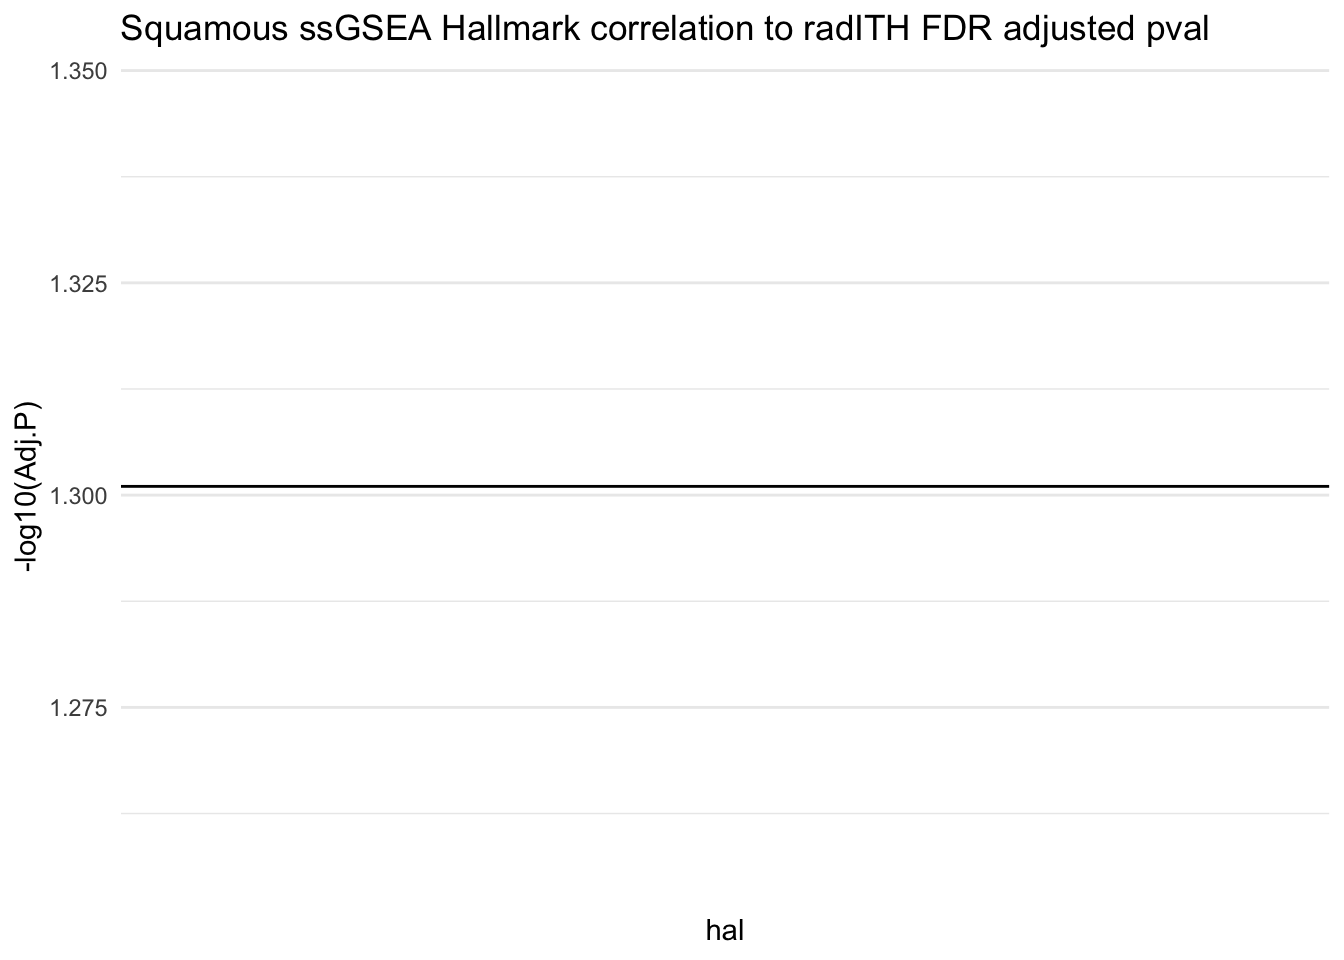
\includegraphics{radiomics_USA_January_2022_files/figure-latex/unnamed-chunk-15-1.pdf}

\section{Hallmark expression-radITH Correlation in Large vs Small tumors
(all
samples)}\label{hallmark-expression-radith-correlation-in-large-vs-small-tumors-all-samples}

-Large tumors seem to harbour association between radITH and biology\\
-Small tumors not significant hits\\
-Using wavelet kernel it was the opposite
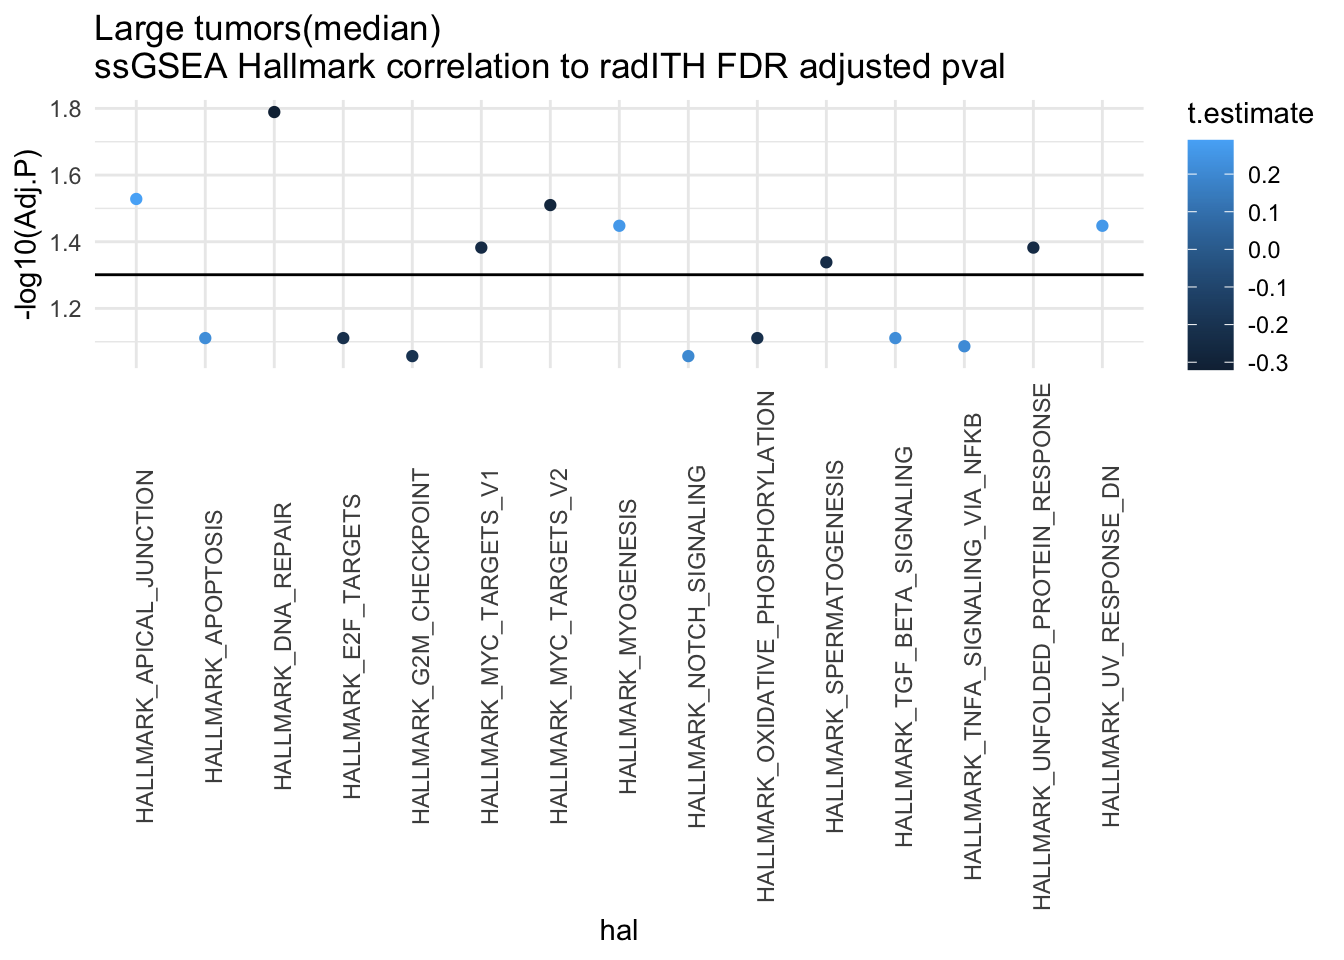
\includegraphics{radiomics_USA_January_2022_files/figure-latex/unnamed-chunk-16-1.pdf}
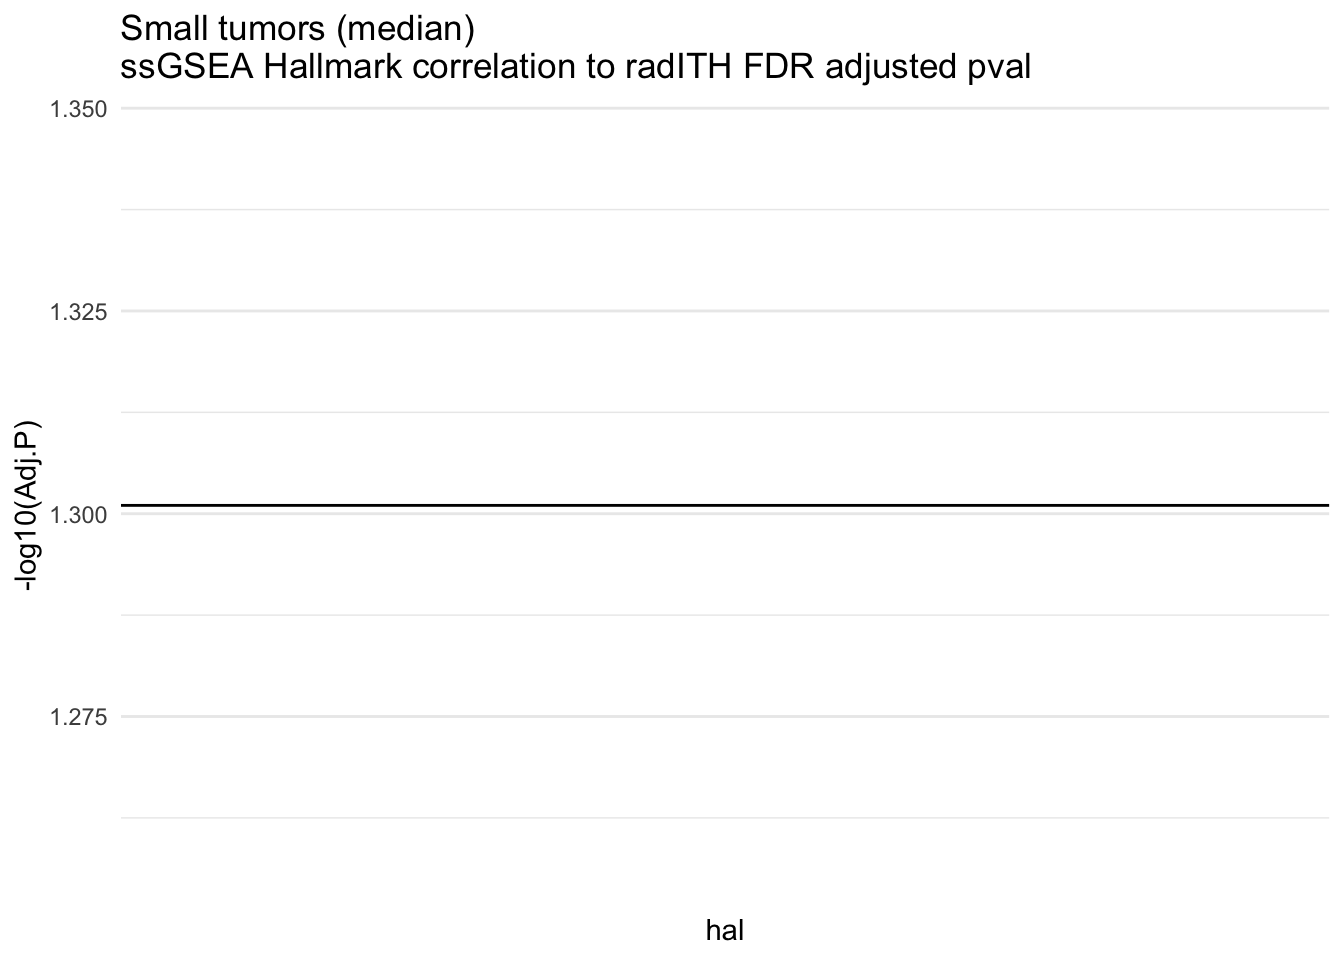
\includegraphics{radiomics_USA_January_2022_files/figure-latex/unnamed-chunk-16-2.pdf}

\section{Let's split by Size and Pathology and
repeat}\label{lets-split-by-size-and-pathology-and-repeat}

-Large Squamous cell tumors show significant hits in DNA repair and MYC
targets v2\\
-Small Squmous, no significant hits -Small/Big Adeno tumors do not show
any significant hits
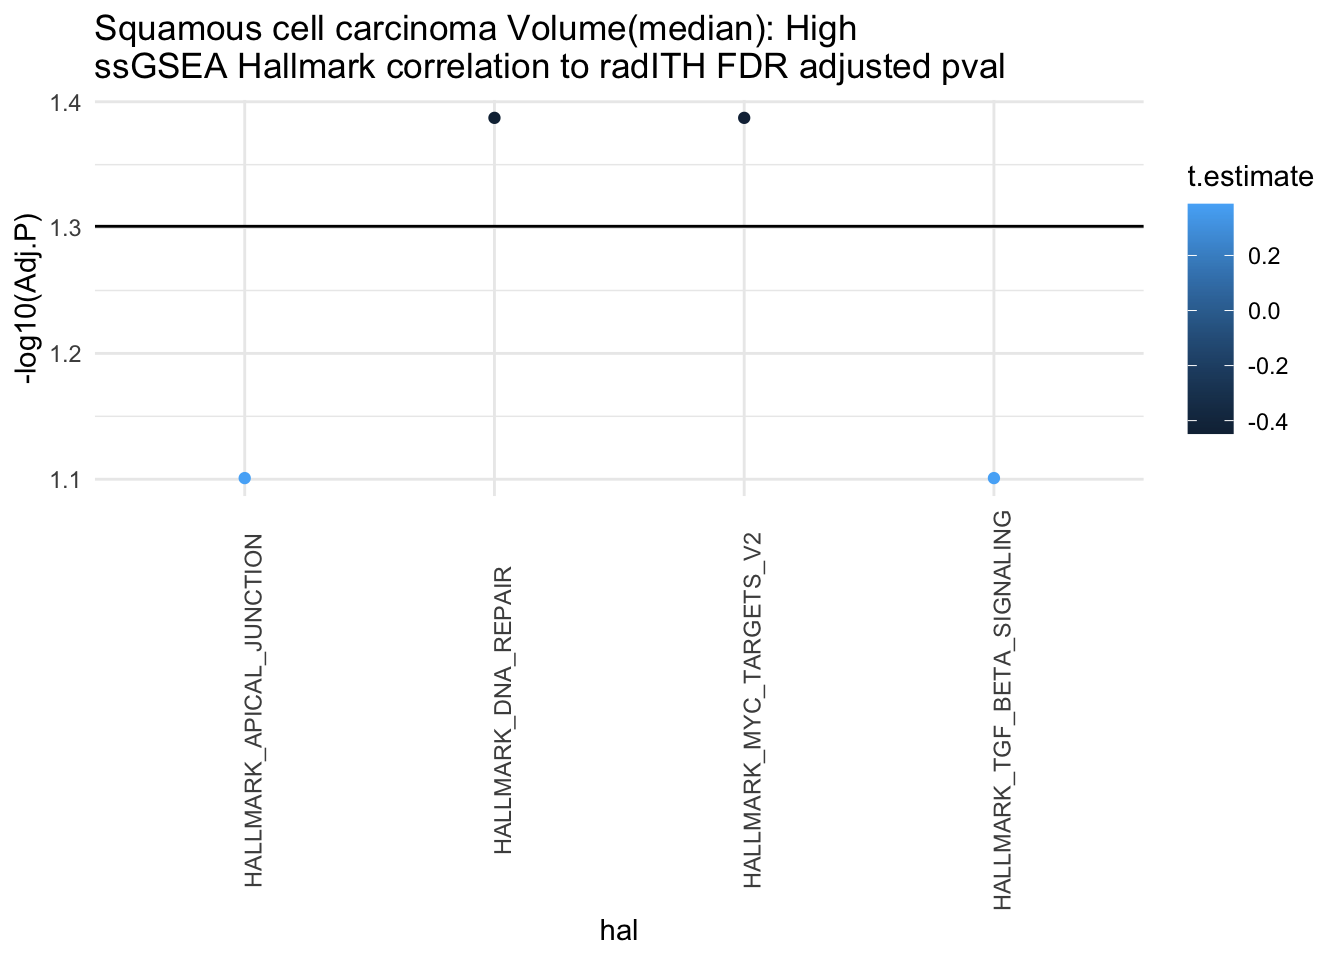
\includegraphics{radiomics_USA_January_2022_files/figure-latex/unnamed-chunk-17-1.pdf}

\end{document}
